\section{Theorie}
\label{sec:Theorie}

\subsection{Fehlerrechnung}

Für die Fehlerfortpflanzung bei Gleichungen mit $N$ fehlerbehafteten Größen
wird jeweils die Formel zur Gaußschen Fehlerfortpflanzung

\begin{equation*}
  \sigma = \sqrt{\sum_{i=1}^{N}\biggl(\frac{\partial f(x_{\g{i}})}{\partial x_{\g{i}}}
  \sigma_{\g{i}}\biggr)^2}
\end{equation*}
mit der jeweiligen Funktion $f(x_{\g{i}})$, den Messgrößen $x_{\g{i}}$ und den
zugehörigen Fehlern $\sigma_i$ verwendet.
Zur Berechnung des arithmetischen Mittels von $N$ Messwerten wird jeweils die
Formel

\begin{equation*}
  \overline{x} = \frac{1}{N}\sum_{i=1}^{N}x_{\g{i}}
\end{equation*}
mit den Messwerten $x_i$ benutzt.
Die Standardabweichung des Mittelwerts wird jeweils mit der Gleichung

\begin{equation*}
  \overline{\sigma} = \sqrt{\frac{1}{N-1}\sum_{i=1}^{N}(x_{\g{i}} - \overline{x})^2}
\end{equation*}
mit den $N$ Messwerten $x_i$ berechnet.

\subsection{Einleitung}

Auf mikroskopischer Skala sind die Ladungsdichte $\rho$ und die Stromdichte $\vec{j}$ in einem Leiter
schwankende Größen. Das ist darin begründet, dass die Elementaradung diskontiniuerlich ist und somit nicht den
ganzen Raum gleichmäßig füllt und sich außerdem die Ladungsträger ungeordnet bewegen. Dies hat zur Folge, dass
mit empfindlichen Messgeräten statistische Schwankungen, das sogenannte Rauschen, in der Spannung $U$ und der
Stromstärke $I$ in einem Schaltkreis detektierbar sind. Im Folgenden werden unterschiedliche Formen
des Rauschens vorgestellt und im Anschluss daran experimentell untersucht.

\subsection{Verschiedene Rauschphänomene}

Unter dem thermischen Rauschen versteht man das Spannungsrauschen an einem ohmschen Widerstand. Durch
ungeordnete Bewegung der Elektronen bei endlicher Temperatur entstehen stellenweise Ladungsüberschüsse
und dadurch messbare Potentialdifferenzen. Ein typischer Spannungsverlauf ist in Abbildung \ref{fig:thermtyp}
skizziert.

\begin{figure}
  \centering
  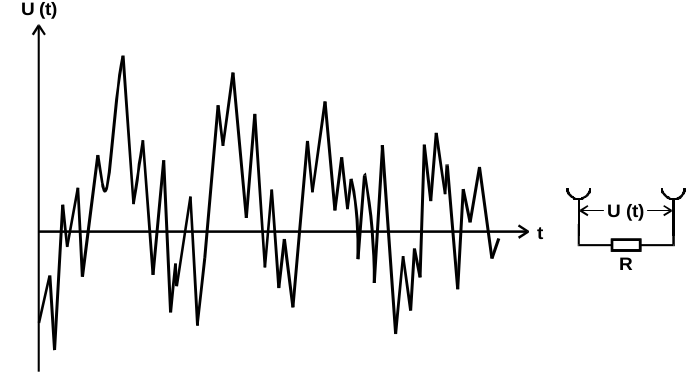
\includegraphics[height=5cm]{Dickpics/thermtyp.png}
  \caption{Ein typischer Spannungsverlauf, der an den Enden eines ohmschen Widerstandes bobachtet werden kann \cite{fig:thermtyp}.}
  \label{fig:thermtyp}
\end{figure}

Das sogenannte Stromrauschen tritt beispielsweise auf, wenn Elektronen aus Festkörperoberflächen emittiert werden.
Dabei wird zwischen zwei Effekten, die für das Rauschen verantwortlich sind, unterschieden.

In einer Diode beispielsweise entsteht ein Stromrauschen, da die an der Kathode emittierten Elektronen in unregelmäßigen Abständen
auf die Anode treffen. Die Abweichungen in der Stromstärke sind zwar klein, können aber mit geeigneten Messgeräten
sichtbar gemacht werden. Das unregelmäßige Auftreffen der Elektronen auf die Anode ist vergleichbar mit dem Auftreffen von Schrotkörnern
auf eine Metallplatte, weshalb dieses Phänomen Schrot-Effekt genannt wird.

Der Funkel-Effekt beschreibt ein Stromrauschen, welches entsteht, wenn die Austrittsarbeit an der Kathode zeitabhängig ist.
Dies spielt vor allem bei Oxydkathoden eine große Rolle und soll in diesem Versuch ebenso wie der Schroteffekt untersucht
werden.

\subsection{Stationäre und Ergodische Schwankungserscheinungen}

Um einen Rauschprozess zu quantifizieren ist es nicht zweckmäßig den genauen Verlauf
von Schwankungen zu untersuchen, da zumindest die im vorangegangenen Abschnitt vorgestellten
Rauschphänomene stochastische, zum Teil indeterministische, Prozesse sind. Stattdessen
werden geeignete Mittelwerte von Rauschströmen bzw. -spannungen untersucht.
Der zeitliche Mittelwert einer Rauschspannung verschwindet i.A., wenn diverse Parameter, zum Beispiel
die Temperatur, konstant gehalten werden. Der quadratische Mittelwert
\begin{align}
  \overline{U^2}(\tau) = \frac1{\tau} \int_{0}^{\tau} U^2(t) \mathrm{d}t
\end{align}
hingegen ist i.A. nicht Null und beinhaltet Informationen über den Rauschprozess im Zeitintervall $[0,\tau]$. Wenn dieser Wert
unabhängig von der Wahl des Zeitintervalls ist, also alle Parameter, die Einfluss auf das Rauschen haben, konstant
gehalten werden, wird die Schwankungserscheinung als stationär bezeichnet.
Das sogenannte Scharmittel
\begin{align}
  \langle U^2(t_0) \rangle = \frac1{N} \sum_{i=1}^{N} U_i^2(t_0)
\end{align}
ergibt sich über Mittelung mehrerer identischer Rauschquellen zum selben Zeitpunkt $t_0$.
Sind Scharmittel und Zeitmittel gleich, so wird die Schwankungserscheinung als ergodisch bezeichnet.
Das ist zum Beispiel beim thermischen Widerstandsrauschen oder beim Schroteffekt der Fall, wenn sämtliche
Parameter wie die Temperatur oder der mittlere Diodenstrom konstant gehalten werden.

Da die vorgestellten Schwankungserscheinungen, wie bereits erwähnt, mikroskopischer Natur sind,
lassen sich mittels verschiedener Messungen mikroskopische Größen bestimmen. So soll in diesem
Versuch die Elementarladung $\mathrm{e}_0$ und die Boltzmannsche Konstante $k_\text{B}$ experimentell durch eine
Rauschmessung bestimmt werden. Dazu werden zunächst theoretische Zusammenhänge für die erwähnten Rauschprozesse hergeleitet.

\subsection{Das Thermische Rauschen und die Nyquist-Beziehung}

Aus einem Gedankenexperiment einer verlustosen Doppelleitung, die durch zwei Widerstände
kurzgeschlossen wird, und diverser Annahmen aus der statistischen Thermodynamik kann eine
Beziehung zwischen dem quadratischen Rauschspannungsmittelwert $\overline{U^2}$ und der Temperatur
$T$ hergeleitet werden. Diese sogenannte Nyquist-Beziehung lautet
\begin{align}
  \overline{U^2} = 4 k_\text{B} \cdot T \cdot R \cdot \Delta \nu. \label{eqn:nyquist}
\end{align}
Dabei ist $R$ der Widerstand der Rauschquelle und $\Delta \nu$ das Frequenzintervall der Rauschspannung. Da
$\overline{U^2}$ nicht dispersiv ist, sondern nur von der Breite des Frequenzintervalls abhängig ist, wird das Rauschen des Widerstands auch weißes Rauschen genannt.
Es ist zu beachten, dass diese Gleichung nur in einem Frequenzbereich von unter $\SI{6e11}{\hertz}$ gilt,
wie in Abbildung \ref{fig:freqab} dargestellt, darüber ist $\overline{U^2}$ dispersiv. Bei Zimmertemperatur gilt jedoch die Relation
$h\nu \ll k_\text{B}T$ und damit auch die Nyquist-Beziehung.

\begin{figure}
  \centering
  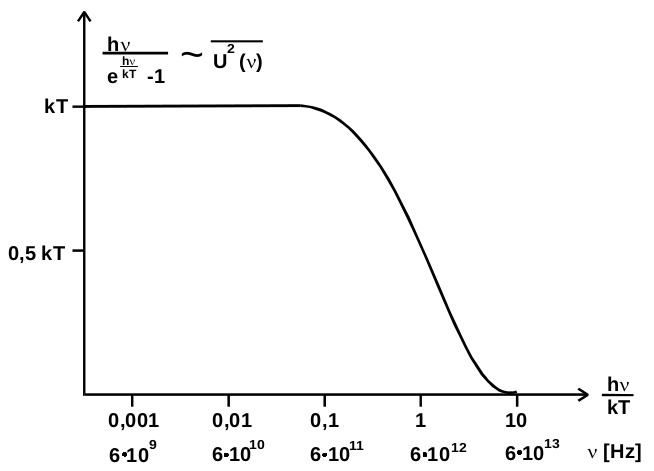
\includegraphics[height=7cm]{Dickpics/freqab.png}
  \caption{Frequenzabhängigkeit des quadratischen Rauschspannungsmittelwerts beim thermischen Widerstandsrauschen \cite{anleitung}.}
  \label{fig:freqab}
\end{figure}

Des Weiteren muss beachtet werden, dass ein realer Widerstand immer eine endliche Eigenkapazität besitzt. Das Ersatzschaltbild
dazu ist in Abbildung \ref{fig:ersatzschaltbildR} zu sehen. Über die Maschenregel folgt das effektive, messbare Spannungsrauschen
\begin{align}
  \overline{U_{\text{RC}}^2} = \overline{U_{\text{R}}^2} \cdot \frac1{1+(2\pi\nu_\text{m} RC)^2},
\end{align}
wobei $\nu_\text{m}$ hier der Mittelwert des betrachteten Frequenzintervalls $\Delta \nu$ ist.

\begin{figure}
  \centering
  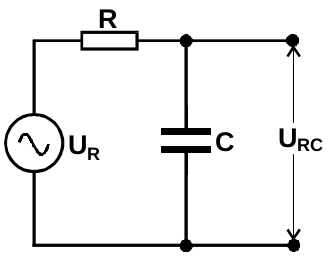
\includegraphics[height=3.7cm]{Dickpics/ersatzschaltbildR.png}
  \caption{Ersatzschaltbild des realen Widerstandes mit einem idealen ohmschen Widerstand $R$ und einer idealen Kapazität $C$ \cite{anleitung}.}
  \label{fig:ersatzschaltbildR}
\end{figure}

\subsection{Das Schrotrauschen und die Schottky-Beziehung}

Zur Messung des Schrotrauschens einer Reinmetallkathode eignet sich die in Abbildung \ref{fig:schrotdiode} skizzierte
Versuchsanordnung. Die Anodenspannung sollte dabei so hoch gewählt sein, dass die Diode im Sättigungsbereich arbeitet,
damit alle an der Kathode emittierten Elektronen die Anode erreichen.
Der gesamte Anodenstrom lässt sich aufspalten in
\begin{align}
  I_\text{ges}(t) = I_0 + I(t),
\end{align}
wobei $I_0$ der mittlere Anoden(gleich)strom und $I(t)$ der Rauschstrom ist, dessen Mittelwert Null ist.
Um eine Beziehung für das mittlere Rauschstromquadrat $\overline{I^2}$ herzuleiten, werden
folgende Annahmen gemacht:
\begin{enumerate}%[(a)]
  \item Die Elektronen werden unabhängig voneinander an der Kathode emittiert.
  \item Die Bewegung der Elektronen auf dem Weg zu Anode wird nicht durch andere Elektronen
  beeinflusst und ist bei allen Elektronen annähernd äquivalent. \\
  $\to$ Sättigungsbereich
  \item Die Elektronen starten mit $v \approx 0$.
  \item Es entstehen keine Sekundärelektronen an der Anode.
\end{enumerate}

\begin{figure}
  \centering
  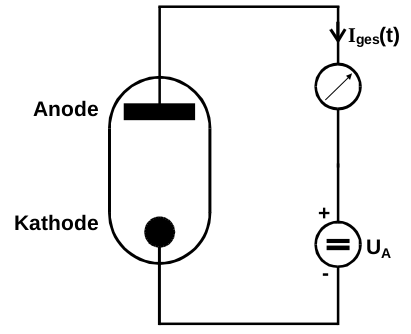
\includegraphics[height=5cm]{Dickpics/schrotdiode.png}
  \caption{Schaltbild der Reinmetalldiode zur Ausmessung des Schrotrauschens \cite{anleitung}.}
  \label{fig:schrotdiode}
\end{figure}

Das zum Zeitpunkt $t_n$ emittierte Elektron induziert durch Influenzwirkung einen Strom
\begin{align}
  I_n(t) = \mathrm{e_0} f(t-t_n)
\end{align}
in der Anode. Die Funktion $f(t-t_n)$ beschreibt dabei die Form des Stromimpulses und ist nur
im Flugzeitintervall $\tau$ von Null verschieden. Der gesamte Anodenstrom ergibt sich durch Summation
gemäß
\begin{align}
  I_\text{ges}(t) = \mathrm{e}_0 \sum_n f(t - t_n).
\end{align}
Durch Ausnutzen des Campbellschen Theorems und der Parsevalidentität folgt die spektrale Verteilungsfunktion des Schrotrauschens
\begin{align}
  W_\text{Schrot}(\nu) = 2 \mathrm{e}_0 I_0 \left| F(\nu) \right|^2.\label{eqn:campbell}
\end{align}
Dabei ist $F(\nu)$ die Fouriertransformierte eines Einzelstromimpulses $f(t)$.
Im Niederfrequenzbereich
\begin{align}
  \nu \ll \frac1{2\pi\tau},
\end{align}
also wenn die Emissionsperiodendauer der Elektronen wesentlich größer als die Flugzeit $\tau \approx \SI{3}{\nano\second}$ der Elektronen ist, gilt
\begin{align}
  F(\nu) \approx 1.
\end{align}
Insgesamt ergibt sich in diesem Bereich
\begin{align}
  \overline{I^2} = 2 \mathrm{e}_0 I_0 \Delta \nu.\label{eqn:schottky}
\end{align}
Diese Relation wird auch Schottky-Beziehung genannt und stellt ebenfalls ein weißes Rauschen dar,
da $\overline{I^2}$ nicht dispersiv ist. Die Voraussetzungen 3. und 4. sind im betrachteten
Niederfrequenzbereich nicht relevant, da spürbare Effekte durch endliche Anfangsgeschwindigkeiten
und Sekundärelektronen erst bei Frequenzen im ausgeschlossenen Bereich $\nu \approx 1/2\pi\tau$ auftreten.
Es ist jedoch essentiel wichtig, dass die Diode im Sättigungsbereich betrieben wird.
Ansonsten wird das Rauschen effektiv abgeschwächt, da dichter bzw. weniger dicht beieinander
emittierte Elektronen eine Raumladung erzeugen, die der Dichteschwankung entgegenwirkt. Es ist daher
zu erwarten, dass $\overline{I^2}$ in diesem Bereich kleiner als durch die Schottky-Beziehung vorausgesagt ist.

\subsection{1/f-Rauschen und der Funkel-Effekt}

Durch Generations-Rekombinations-Prozesse von Ladungsträgern in Oxid-Halbleiter-Grenzschichten entstehen
Rauschströme, deren spektrale Leistungsdichte in bestimmten Frequenzbereichen proportional zur reziproken Frequenz ist.
Allgemein lässt sich herleiten, dass die spektrale Leistungsdichte für das sogenannte Generations-Rekombinations-Rauschen
\begin{align}
  W_\tau(\nu) = \text{const} \frac{\tau}{1+(2 \pi \nu \tau)^2}
\end{align}
ist, wobei $\tau$ die Relaxationszeitkonstante für einen Generations-Rekombinations-Prozess ist.
Für $\nu \ll 1/\tau$ ist $W_\tau(\nu)$ nicht dispersiv, es liegt also weißes Rauschen vor.
Sobald $\nu \propto 1/\tau$ fällt die spektrale Leistungsdichte ab, wie auch den gestrichelten Linien
in Abbildung \ref{fig:leistungsdichte} entnehmbar ist. Wenn die Relaxationszeit variabel ist, wie es in der
Realität auch der Fall ist, dann ist dieser Abfall der Leistungsdichte proportional zur reziproken Frequenz
und es liegt ein 1/f-Rauschen vor.

\begin{figure}
  \centering
  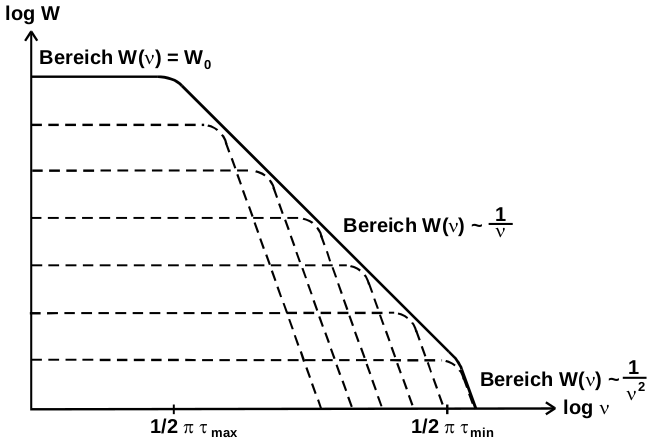
\includegraphics[height=6.5cm]{Dickpics/leistungsdichte.png}
  \caption{Schematischer Verlauf der spektralen Leistungsdichte beim Generations-Rekombinations-Rauschen. Die gestrichelten Linien
  beschreiben den Verlauf bei fester Relaxationszeit $\tau$. Liegt $\tau$ variabel in einem Intervall $[\tau_\text{min}, \tau_\text{max}]$
  so ergibt sich ein 1/f-Rauschen, hier dargestellt durch die durchgezogene Linie \cite{anleitung}.}
  \label{fig:leistungsdichte}
\end{figure}

Nimmt man für die Relaxationszeit $\tau$ einen exponentiellen Zusammenhang
\begin{align}
  \tau(E) = \tau_0 \text{exp}\left(\frac{E}{k_\text{B}T}\right)
\end{align}
zur Aktivierungsenergie $E$ eines Generations-Rekombinations-Prozesses an, so ergibt sich die spektrale Leistungsdichte
\begin{align}
  W(\nu) = \frac{\text{const} k_\text{B} T}{\nu} \left\{ \arctan{(2\pi\nu\tau_\text{min})} - \arctan{(2\pi\nu\tau_\text{max})} \right\}.
\end{align}
Die Werte $\tau_\text{min}$ bzw. $\tau_\text{max}$ beschränken die Relaxationszeit auf ein Intervall, wie auch
die Aktivierungsenergie auf ein Intervall $[E_\text{min}, E_\text{max}]$ beschränkt ist.
Es können nun anhand der Grenzfälle
\begin{align}
  \arctan{(x)} &\to x \qquad \, \text{für} &x &\to 0 \\
  \arctan{(x)} &\to \frac{\pi}{2} \qquad \text{für} &x &\to \infty
\end{align}
qualitativ drei Frequenzbereiche unterschieden werden:
\begin{enumerate}
  \item Für $2\pi\nu\tau \ll 1$ resultiert keine Frequenzabhängigkeit und daher weißes Rauschen.
  \item Für $2\pi\nu\tau_\text{min} \ll 1$ und $2\pi\nu\tau_\text{max} \gg 1$ resultiert
  \begin{align}
    W(\nu) = \frac{\text{const} k_\text{B} T}{\nu} \frac{\pi}{2}
  \end{align}
  und daher 1/f-Rauschen.
  \item Für $2\pi\nu\tau \gg 1$ resultiert eine $1/\nu^2$-Abhängigkeit.
\end{enumerate}
Ein 1/f-Rauschen entsteht beispielsweise an einer Oxid-Metall-Kathode durch eine sich zeitlich ändernde Austrittsarbeit,
was wie bereits erwähnt als Funkel-Effekt bezeichnet wird. Dieses Rauschen überlagert sich mit dem weißen Schrotrauschen, das
im vorangegangenen Kapitel behandelt wurde.
Abhängig vom Diodenstrommittelwert $I_0$ ergibt sich für das Frequenzspektrum des Rauschens durch den Funkeleffekt
\begin{align}
  W_\text{Funkel}(\nu) = \frac{\text{const} I_0^2}{\nu^\alpha},
\end{align}
wobei $\alpha \approx 1$.

\subsection{Versuchsaufbauten zur Ausmessung des thermischen Widerstandsrauschen}

In Abbildung \ref{fig:rauschspektro} ist das Blockschaltbild eines einfachen Rauschspektrometers skizziert.

\begin{figure}
  \centering
  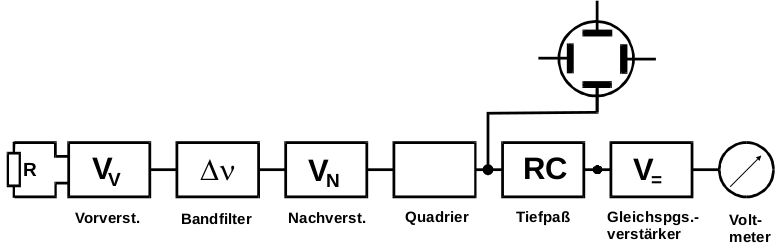
\includegraphics[height=4cm]{Dickpics/rauschspektro.png}
  \caption{Blockschaltbild eines einfachen Rauschspektrometers \cite{anleitung}.}
  \label{fig:rauschspektro}
\end{figure}

Die Amplituden der Rauschspannungssignale am Widerstand $R$ werden zunächst im Vorverstärker mit dem Faktor $V_\text{V}$ linear verstärkt
und daraufhin am Bandfilter diejenigen Frequenzen herausgefiltert, die außerhalb des Frequenzintervalls $\Delta \nu$ liegen.
Die übrigen Signale werden im Nachverstärker um den Faktor $V_\text{N}$ nachverstärkt und an einen Quadrierer weitergegeben,
welcher aus den eintreffenden Spannungssignalen das Signal $V_\text{V}^2 V_\text{N}^2 U_R^2(t)$ bildet. Dieses läuft anschließend
in einen Tiefpass, wo der Gleichspannungsanteil herausgefiltert wird, und kann, nachdem es in einem Gleichspannungsvertärker
mit $V_=$ verstärkt wird, am Voltmeter gemessen werden. Im Idealfall wird also die Größe
\begin{align}
  U_\text{A}^2 = V_= V_\text{V}^2 V_\text{N}^2 \overline{U_R^2} = V_= V_\text{V}^2 V_\text{N}^2 \Delta \nu 4 k_\text{B} T R
  \label{eqn:Uarauschspektro}
\end{align}
gemessen. Dabei ist $V_\text{V}^2 V_\text{N}^2 \Delta \nu$ eine Apparaturkonstante, die durch eine Eichmessung bestimmt werden kann, sodass
zuletzt die Boltzmannkonstante $k_\text{B}$ bestimmt werden kann. Gleichung \eqref{eqn:Uarauschspektro} gilt jedoch nur im Falle
idealer Apparaturen. In der Realität produzieren alle Bauteile Rauschspannungen, die sich mit der des Widerstands überlagern und das
Ergebnis verfälschen. Das fällt vor allem beim Vorverstärker ins Gewicht, da dessen Eigenrauschen insgesamt am stärksten nachverstärkt wird.
Indem ein Nullwiderstand, anstatt des ohmschen Widerstandes $R$ am Eingang des Rauschspektrometers angeschlossen wird, kann eine Abschätzung
des Apparatureigenrauschens gemacht werden und falls nötig Messwerte um einen Offset korrigiert werden.
Dazu ist ein Ersatzschaldbild für einen Verstärker mit Eigenrauschen in Abbildung \ref{fig:verstärkerrauschen} dargestellt.

\begin{figure}
  \centering
  \includegraphics[height=5cm]{Dickpics/verstärkerrauschen}
  \caption{Ersatzschaltbild eines Verstärkers mit Eigenrauschen \cite{anleitung}.}
  \label{fig:verstärkerrauschen}
\end{figure}

Nimmt man gemäß der Abbildung die Spannung
\begin{align}
  U_1(t) = U_R(t) + U(t) + I(t)
\end{align}
am Eingang des Vorverstärkers an, so ergibt sich am Ausgang des Rauschspektrometers
\begin{align}
  U_\text{A}^2 = V_\text{ges}^2 \overline{U_R^2} + V_\text{ges}^2 \left( R^2 \overline{I^2} + 2 R \overline{U I} + \overline{U^2} \right) \approx V_\text{ges}^2 \overline{U_R^2} + V_\text{ges}^2 \overline{U^2},
\end{align}
wobei die Näherung für die im Versuch vorliegenden Vorverstärker mit MOS-Feldeffekttransistoren gerechtfertigt ist.
Die Messung des Verstärkerrauschterms $V_\text{ges}^2 \overline{U^2}$ erfolgt, wie bereits erwähnt, durch Kurzschließen des
Rauschspektrometereingangs.

Für Verstärkerrauschspannungen $|U| \gg |U_R|$ wird das im vorangegangenen Teil beschriebene Verfahren ungenau und es eignet sich
anstatt dessen die in Abbildung \ref{fig:korrelatorschaltung} dargestellte, sogenannte Korrelatorschaltung.

\begin{figure}
  \centering
  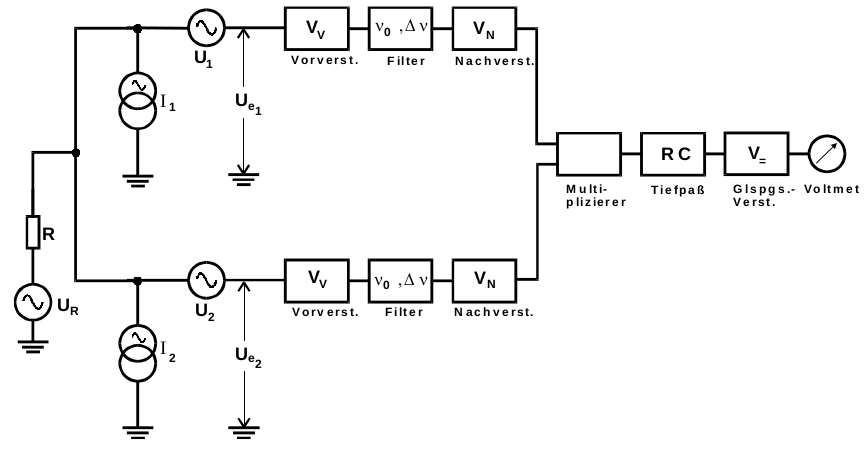
\includegraphics[height=7.3cm]{Dickpics/korrelatorschaltung.png}
  \caption{Blockschaltbild der Korrelatorschaltung zur Ausmessung des thermischen Widerstandsrauschens \cite{anleitung}.}
  \label{fig:korrelatorschaltung}
\end{figure}

Bei dieser Schaltung ergibt sich die Ausgangsspannung zu
\begin{align}
  U_\text{A,korr}^2 = V_\text{ges}^2 \left \{ \overline{U_R^2} + R \left( \overline{U_1 I_1} + \overline{U_2 I_2} \right) + R^2 \left( \overline{I_1^2} + \overline{I_2^2} \right) \right \} \approx V_\text{ges}^2 \overline{U_R^2},
\end{align}
sofern erneut Vorverstärker mit MOS-Feldeffekttransistoren verwendet werden. Das Verstärkerrauschen ist also näherungsweise Null, obwohl
mit dieser Schaltung dieselbe Verstärkung erreicht werden kann.

Mit Hilfe der Rauschzahl
\begin{align}
  F(\nu_0,Z) = \frac{\overline{U_\text{A}^2}(Z)}{4 k_\text{B} T \Delta \nu V_\text{ges}^2 \cdot \text{Re}(Z)}\label{eqn:rauschzahl}
\end{align}
können Aussagen über das Eigenrauschen und damit über die Qualität eines Verstärkers abhängig von der
Lage $\nu_0$ des Durchlassbereichs und dem Wellenwiderstand $Z$ des angeschlossenen Rauschelements gemacht werden.
Der niedrigste und gleichzeitig optimalste Wert für die Rauschzahl ist $F = 1$.




\cite{anleitung}
